% -----------------------------------------------------------------------
% --- DOCUMENT ---
% -----------------------------------------------------------------------

\documentclass[11pt, a4paper, french, twoside]{article}



% -----------------------------------------------------------------------
% --- PACKAGE ---
% -----------------------------------------------------------------------
\usepackage[french]{babel}

% Font
\usepackage[utf8]{inputenc}
\usepackage[T1]{fontenc}

% Marge du document
\usepackage[top=3.5cm,
            bottom=3cm,
            left=2cm,
            right=2cm,
            footskip=1.5cm,
            headheight=1.5cm,
            headsep=0.9cm]{geometry}

% Gérer les positionnement d'images
\usepackage{float}

% Import de fichier externe
\usepackage{graphicx}

% Mise en forme des URL
\usepackage{url}

% Informations sur un document compilé en PDF et les liens externes / internes
\usepackage{hyperref}


% Mise en page des tableaux
\usepackage{array}
\usepackage{tabularx}

% Espacement entre les lignes
\usepackage{setspace}

% Modifier la mise en page de l'abstract
\usepackage{abstract}

\usepackage{titlesec}

% Pour les entêtes
\usepackage{fancyhdr}

% Pour l'import de code
\usepackage{listings}

% Utilisation de couleur
\usepackage{color}

%pour utiliser \floatbarrier
%\usepackage{placeins}
%\usepackage{floatrow}

% Pour voir les mages
%\usepackage{layout}
%\layout

% Annexes
\usepackage{appendix}

% Ajouter un glossaire
\usepackage[toc]{glossaries}
\makeglossary
\loadglsentries{glossaire}

% Ne pas supprimer, permet d'afficher le numéro de sections
\usepackage{etoolbox}

\makeatletter
\patchcmd{\ttlh@hang}{\parindent\z@}{\parindent\z@\leavevmode}{}{}
\patchcmd{\ttlh@hang}{\noindent}{}{}{}
\makeatother


% -----------------------------------------------------------------------
% --- Couleurs définies
% -----------------------------------------------------------------------
\definecolor{pblue}{rgb}{0.13,0.13,1}
\definecolor{pgreen}{rgb}{0,0.5,0}
\definecolor{pred}{rgb}{0.9,0,0}
\definecolor{pgrey}{rgb}{0.46,0.45,0.48}
\definecolor{backcolour}{gray}{0.95}


% -----------------------------------------------------------------------
% --- Listing de code
% -----------------------------------------------------------------------
\lstset{language=Java,
    basicstyle=\tiny,
    backgroundcolor=\color{backcolour},
    showspaces=false,
    showtabs=false,
    breaklines=true,
    xleftmargin=0.5cm,
    framexleftmargin=0.5cm,
    framextopmargin=6pt,
    framexbottommargin=6pt,
    frame=tb,
    framerule=0pt,
    showstringspaces=false,
    breakatwhitespace=true,
    commentstyle=\color{pgreen},
    keywordstyle=\color{pblue},
    stringstyle=\color{pred},
    basicstyle=\ttfamily,
    moredelim=[is][\textcolor{pgrey}]{\%\%}{\%\%}
}



% -----------------------------------------------------------------------
% --- INFORMATION SUR LE DOCUMENT
% -----------------------------------------------------------------------

% Information sur le document
\hypersetup{
    pdfauthor = {
        Edward Ransome,
        Guillaume Milani,
        Mathieu Monteverde,
        Michael Spierer,
        Sathiya Kirushnapillai},                    % Auteurs
    pdftitle = {GEMMS - Editeur d'image},           % Titre du document
    pdfsubject = {Mémoire de Projet},               % Sujet
    pdfkeywords = {Tag1, Tag2, Tag3, ...},          % Mots-clefs
    pdfstartview={FitH}}                            % ajuste la page à la largueur de l'écran
%pdfcreator = {MikTeX},                             % Logiciel qui a crée le document
%pdfproducer = {}}                                  % Société avec produit le logiciel



% -----------------------------------------------------------------------
% --- EN-TETE ET PIED DE PAGE ---
% -----------------------------------------------------------------------
\pagestyle{fancy}
\fancyhf{} % Supprime les entetes et pieds de page existants

\fancyhead[LE,RO]{Projet de semestre\\}
\fancyhead[RE,LO]{IL - TIC - HEIG-VD \\ Printemps 2017}
\fancyfoot[LE,RO]{\thepage{}}
\fancyfoot[RE]{G. Milani, E. Ransome, M. Monteverde, M. Spierer, S. Kirushnapillai}
\fancyfoot[LO]{Éditeur d'images GEMMS}
\renewcommand{\footrulewidth}{1pt}


\title{Éditeur d'images GEMMS \\ Rapport}
\author{G. Milani, E. Ransome, M.Monteverde, M. Spierer, S. Kirushnapillai}
\date{Mars 2017}



% -----------------------------------------------------------------------
% --- DEBUT DU DOCUMENT ---
% -----------------------------------------------------------------------
\begin{document}
\selectlanguage{french}
\graphicspath{ {img/} }

% Espacement entre les lignes
\newcommand{\HRule}{\rule{\linewidth}{0.5mm}}

% Page de garde
\begin{titlepage}
    \begin{center}
        % Upper part of the page. The '~' is needed because only works if a paragraph has started.
        % \includegraphics[width=0.35\textwidth]{./logo}~\\[1cm]
        
        \textsc{\LARGE Haute Ecole d'Ingénierie et de Gestion du Canton de Vaud (HEIG-VD)}\\[1.5cm]
        
        \textsc{\Large }\\[0.5cm]
        
        % Title
        \HRule \\[0.4cm]
        
        {\huge \bfseries Projet de semestre (PRO)\\
            Editeur d'image GEMMS \\[0.4cm] }
        
        \HRule \\[1.5cm]
        
        % Author and supervisor
        \begin{minipage}{0.4\textwidth}
            \begin{flushleft} \large
                \emph{Auteur:}\\
                Edward \textsc{Ransome}\\
                Guillaume \textsc{Milani}\\
                Mathieu \textsc{Monteverde}\\
                Michael \textsc{Spierer}\\
                Sathiya \textsc{Kirushnapillai}
            \end{flushleft}
        \end{minipage}
        \begin{minipage}{0.4\textwidth}
            \begin{flushright} \large
                \emph{Client:} \\
                René \textsc{Rentsch}\\
                \emph{Référent:} \\
                René \textsc{Rentsch}\\
            \end{flushright}
        \end{minipage}
        
        \vfill
        
        % Bottom of the page
        {\large \today}
        
    \end{center}
\end{titlepage}

\newpage~


\thispagestyle{empty}
\newpage


% Table des matières
\tableofcontents
\newpage


% Espacement entre les lignes d'un tableau
\renewcommand{\arraystretch}{1.5}

% Config des pages
\setlength{\parskip}{1em}
\setlength{\parindent}{0pt}

\titlespacing\section{0pt}{12pt plus 4pt minus 2pt}{0pt plus 2pt minus 2pt}
\titlespacing\subsection{0pt}{12pt plus 4pt minus 2pt}{0pt plus 2pt minus 2pt}
\titlespacing\subsubsection{0pt}{12pt plus 4pt minus 2pt}{0pt plus 2pt minus 2pt}


~
\thispagestyle{empty}
% Recommencer la numérotation des pages à "1"
\setcounter{page}{0}
\newpage

%====================== INCLUSION DES PARTIES ======================

\section{Introduction}
GEMMS est un éditeur d'images réalisé en Java en se basant sur les fonctionnalités graphiques de JavaFX 8. Il a été réalisé dans le cadre de la branche PRO (Projet de semestre) de la deuxième année d'informatique logicielle de la Haute-École d'Ingénierie et Gestion du canton de Vaud (HEIG-VD). 
Le programme a été élaboré sur une durée de 14 semaines aboutissant le 31 Mai 2017.

\section{Objectif}
L'application GEMMS a été conçue pour éditer des images de manière rapide, simple et intuitive. Le programme ne nécessite pas d'apprentissage particulier, comme certains programmes plus lourds comme Adobe Photoshop ou encore GIMP.

L'interface est propre, avec des icônes représentant les différents outils et actions possibles dans le programme en essayant de minimiser les menus déroulants surchargés. Des infobulles donnent une description concise de chaque outil lorsqu'on passe la souris dessus.

Bien que plus simple que les applications lourdes mentionnées ci-dessus, un concept très important dans l'édition d'image, les calques, est conservé. Certains éditeurs très basiques comme Paint sous Windows ne fournissent pas cette fonctionnalité. Les calques permettent de superposer des images, du texte, ou des canevas et de les déplacer, modifier ou effacer indépendamment les uns des autres. Lors de l'exportation du projet vers un format image, les calques sont aplatis et l'image est exportée en perdant ces informations.

Un projet GEMMS ne peut cependant pas uniquement être exporté en tant qu'image, mais sauvegardée dans un fichier de projet \og.gemms \fg{}. Ce type de fichier peut être ouvert par l'application pour restaurer tout le projet en cours, recréant chaque calque ainsi que les transformations effectuées dessus.

\section{Conception \& Architecture}
\subsection{Technologies utilisées}
\subsubsection{Java 8}
Parmi les deux langages de haut niveau proposés pour l'élaboration de ce projet (Java ou C++), nous avons choisi Java pour sa portabilité, sa sécurité et ses performances. De plus, la dernière version de Java propose la librairie graphique JavaFX qui correspond en tout point à notre projet. Enfin, notre équipe est également plus habile à programmer à l'aide du langage Java.

\subsubsection{JavaFX 8}
JavaFX, successeur de Swing, est la librairie de création d'interface graphiques officielle de Java. La version 8, utilisée pour ce projet, ajoute de nouvelles fonctionnalités et est la plus récente version utilisable avec Scene Builder.

\begin{figure}[h]
    \caption{Architecture de JavaFX}
    \centering
    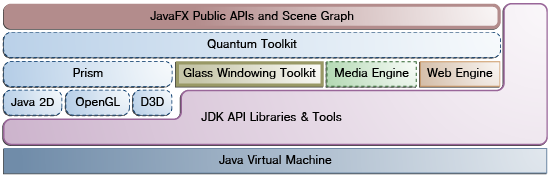
\includegraphics[width=\textwidth]{arch_javafx.png}
    \label{fig:arch_javafx}
\end{figure}

Comme vous pouvez le voir sur la figure \ref{fig:arch_javafx}, BLA BLA BLA A COMPLETER, A PARLER DE CSS ETC


\subsubsection{Scene Builder 8.3.0}
Scene Builder de Gluon permet de manipuler des objets JavaFX graphiquement et exporter ceux-ci dans un fichier .fxml interprétable par la librairie graphique. L'interface de base à été conçue lors de l'élaboration du cahier des charges pour présenter un exemple de l'interface de l'application finale. Plusieurs mock-ups ont été présentés et c'est sur ceux-cis que nous nous sommes basés pour construire, grâce à Scene Builder, une base d'interface sur la laquelle nous avons rajouté des composants et fonctionnalités tout au long de l'élaboration de l'application. La flexibilité de JavaFX permet d'ajouter des éléments via un fichier externe fxml mais aussi directement dans le code, ce que nous avons aussi utilisé.

\subsubsection{Maven}
Pour la compilation du projet et l'importation aisée de celui-ci dans un nouvel environnement de travail, nous avons utilisé l'outil Maven de Apache.
TODO TODO TODO TODO TODO COMPLETER

\subsubsection{Git}
Git est un logiciel de gestion de version utilisé pour permettre de stocker tous les fichiers du projet ainsi que toutes les modifications leur ayant été apportés depuis leur création. Pour chaque nouvelle fonctionnalité, nous avons procédé par la création d'une branche à partir de la branche principale (une version fonctionnelle du programme, contenant les fonctionnalités implémentées et testées). Ces nouvelles branches permettent de développer les fonctionnalités du programme indépendamment et de les ajouter à la branche principale une fois inspectées et testées par plusieurs membres de l'équipe.

\subsubsection{GitHub}
Github est un service web permettant de parcourir visuellement l'historique Git ainsi que de fournir des outils de gestion de Git. Notamment, pour chaque fonctionnalité ou chaque bug découvert, une "issue" (un problème) peut être ouverte et assignée à un ou plusieurs membres de l'équipe. Dès la fin de l'élaboration du planning de notre projet, des issues ont été assignées à chaque développeur. Celles-ci ont permis de mieux se fier au planning et toujours avoir en vue ce qu'il restait à implémenter.

\subsection{Comparaison de l'interface finale avec notre mock-up}
Le mock-up de l'interface à été conçu au début du projet en prenant compte de toutes les fonctionnalités que le programme devait fournir. Voici une comparaison de celui-ci avec l'interface finale.

\begin{figure}[H]
	\caption{Mock-up de l'interface}
	\centering
	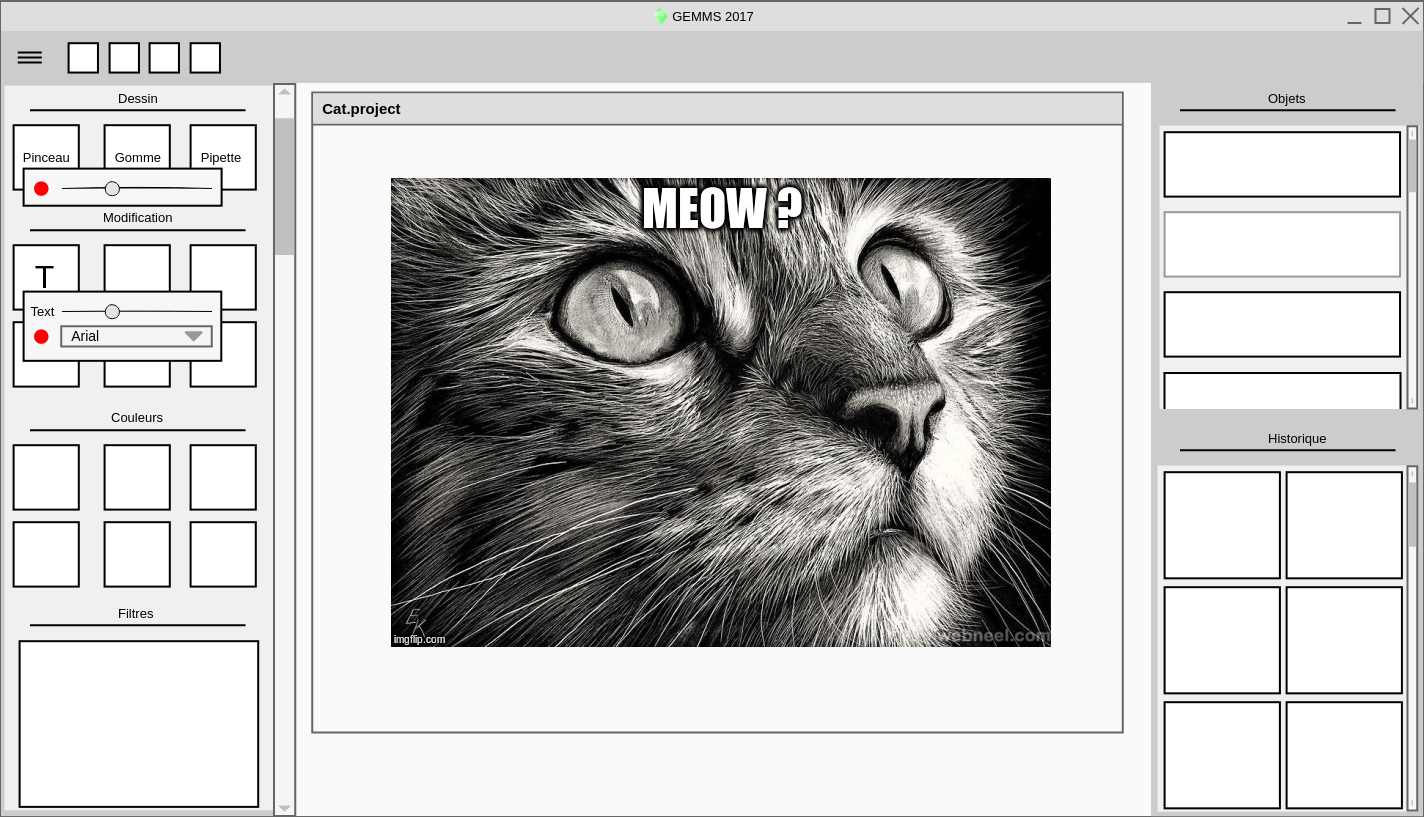
\includegraphics[scale=0.35]{Cat_MOCKUP.png}
	\label{fig:cat_mockup}
\end{figure}

\begin{figure}[H]
	\caption{Interface finale du programme}
	\centering
	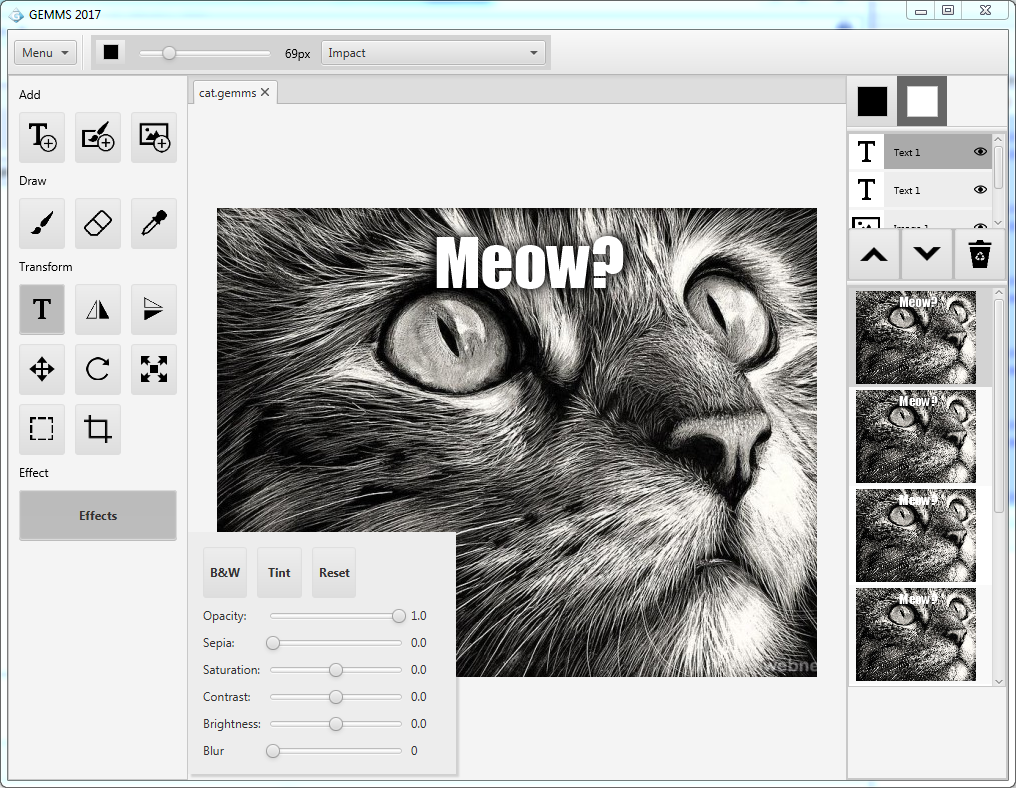
\includegraphics[scale=0.6]{Cat_GEMMS.PNG}
	\label{fig:cat_gemms}
\end{figure}

Comme le montrent les figures \ref{fig:cat_mockup} et \ref{fig:cat_gemms}, l'interface conçue lors de l'élaboration du cahier des charges à été repris presque entièrement pour notre programme. Les différences majeurs sont les paramétrages des outils, qui ont lieux en haut de l'interface à coté du menu déroulant, ainsi que les filtres \& effets, qui ont lieux dans une fenêtre qui peut être ouverte ou fermée à souhait pour rendre l'interface moins chargée. 

\section{Description technique}

Comme cité précédemment, notre application a été codé à l'aide de la librairie JavaFX. Ainsi, toute notre implémentation technique est basée sur cette dernière. 

\subsection{Structure}
JavaFX utilise des fichiers FXML pour séparer la logique de la vue TODO TODO TODO
ImageView, Canvas et Text
Controller

\subsection{Serialisation}
En Java, la sérialisation s'effectue à l'aide de l'interface \og Serializable \fg{}. Par conséquent, chaque classes de Java implémentant cette dernière telle que \og String \fg{}, peut être sérialisé et désérialisé à volonté. Cependant, la majorité des classes JavaFX n'implémente pas cette interface. En effet, cette librairie utilise grandement des mécanismes et des liaisons dynamiques tel que les listeners qui sont pour l'instant des sous-systèmes non-sérialisable. C'est pourquoi, JavaFX contient peu d'objet sérialisable.

Pour combler ce manque, nous devons nous même implémenter la sérialisation des classes JavaFX que nous sommes susceptible d'utiliser. 

\begin{figure}[h]
    \caption{Diagramme de la sérialisation simplifié}
    \centering
    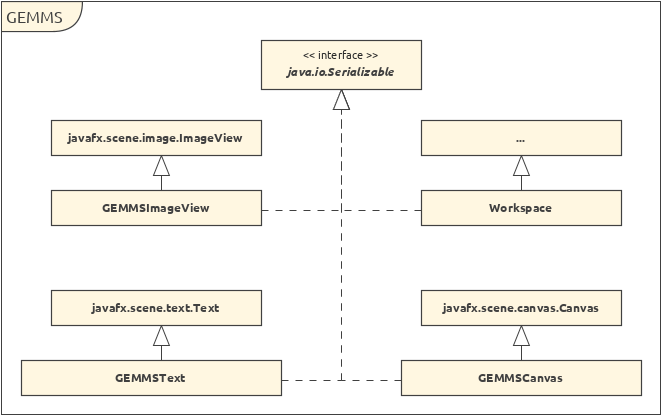
\includegraphics[scale=0.6]{serialisation_diagram.png}
    \label{fig:seri_diag}
\end{figure}

Sur la figure \ref{fig:seri_diag}, nous pouvons voir un diagramme simplifié de l'implémentation de la sérialisation. Dans notre application, nous allons utilisé des classes de base telles que ImageView, Text, Canvas, Color, etc. Nous devons donc spécialiser ces classes afin qu'elles puissent implémenter l'interface \og Serializable \fg{}. Toutefois, certaines classes comme \og Color \fg{} ne sont malheureusement pas spécialisable. Il faut donc sérialiser les paramètres un par un à l'aide des accesseurs et mutateurs de cette dernière.

Étant donné que les classes JavaFX possèdent énormément de fonctionnalités, sérialiser l'entier de celles-ci nous demanderait beaucoup trop de temps. C'est pourquoi nous nous contentons uniquement des paramètres utilisés au sein du projet tel que la largeur, la hauteur, la position, etc. 

\lstinputlisting[language=Java, caption=Exemple de sérialisation]{./src/serialisation.java}

Bien que la sérialisation soit possible, ceci engendre des contraintes et des pertes de performances. Par exemple, les classes spécialisées ne peuvent plus étendre d'une classe commune et bénéficier de ses méthodes. De plus, les objets comme Canvas et ImageView devront sérialiser pixel par pixel, ce qui peut être long et volumineux selon la taille.

\subsection{Sauvegarde}
La sauvegarde d'un document utilise la sérialisation des objets. Comme mentionné précédemment, la sérialisation de certaines classes peut être volumineux. Ainsi, les données sont compressées dans le format GZIP.

\subsection{Workspace et liste des calques}
TODO TODO TODO

\subsection{Copier-coller}
TODO TODO TODO

\subsection{Historique}
Pour garder un historique de chaque action effectuée, on utilise la sérialisation des composants présentée précédemment. A la fin de chaque action modifiant l'espace de travail, une fonction va être appelée permettant de sauvegarder intégralement l'espace de travail courant et le placer sur une pile. A chaque détection de la commande Ctrl + Z, la sauvegarde sera chargée et la modification sera donc effacée. De même, à la détection de la commande Ctrl + Y, on va charger un espace de travail plus récent (s'il y en à un, c'est-à-dire si le Ctrl + Y était précédé d'un Ctrl + Z).

\subsection{Positionnement}
TODO TODO TODO

\subsection{Outils}
\par
JavaFX offre (entre autres) les événements MousePressed, MouseDragged et MouseReleased. Ils correspondent respectivement à l'action de presser la souris, de la déplacer en gardant le clic gauche enfoncé ou de relâcher le clic gauche de la souris. 
\subsubsection{Hiérarchie des outils}
\par
La plupart des outils de l'application  fonctionnent grâce à ces trois événements. On pensera notamment au pinceau qui doit dessiner un trait en suivant la souris lors d'un MouseDragged. 
\par
Comme on peut le voir sur la figure \ref{fig:tool_hier}, les outils implémentent une interface Tool, possédant des méthodes correspondant à ces événements. Au long de l'exécution du programme, le Workspace garde une référence vers un outil considéré actif (qui peut aussi être référence nulle), et lorsqu'il détecte un des événements cités plus haut, il se charge d'appeler la ou les méthodes correspondantes de cet outil.
\par
Lorsque l'utilisateur clique sur un bouton pour activer un outil, le programme crée une nouvelle instance de ce type d'outil, et le Workspace utilise cet outil pour traiter les événement MousePressed, MouseDragged ou MouseReleased.
\par
D'autres outils plus simples, comme la symétrie horizontale ou verticale ou les effets de couleurs sont implémentés en ajoutant un action à des composants de bases de JavaFX comme des Button ou des Slider.
	
\begin{figure}[h]
	\caption{Diagramme simplifié de la hiérarchie des outils}
	\centering
	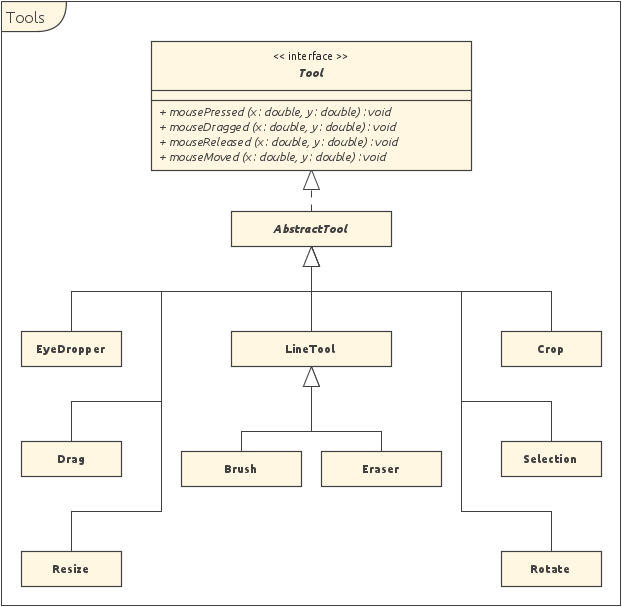
\includegraphics[scale=0.6]{tool_hierarchy.png}
	\label{fig:tool_hier}
\end{figure}

\subsubsection{Réglage des outils}
Certains de ces outils nécessitent d'être paramétrés en temps réel en fonction des calques sélectionnés par l'utilisateur. Par exemple, la taille de la gomme est stockée dans l'objet représentant l'outil, et est utilisée pour déterminer la taille du rectangle à effacer. L'utilisateur peut la régler au moyen d'un Slider (il s'agit d'un composant JavaFX). Les même besoin concernent la gestion de la couleur du pinceau, de la taille et de la police de l'outil de modification de texte.
\par
Ces réglages doivent pouvoir s'adapter à un outil existant, comme par exemple récupérer la taille actuelle du pinceau et la garder en mémoire.

Pour ce faire, les réglages sont gérés au moyen d'une hiérarchie de classes (se référer à la figure \ref{tool_settings}), qui sont en fait des spécialisations de composants JavaFX permettant à l'utilisateur de paramétrer les outils, et d'une série d'interfaces représentant des outils pouvant être paramétrés sur divers aspects (la taille, la couleur, la police et ainsi de suite).
\par
Ainsi un objet ToolSizeSettings est un élément graphique de contrôle qui contient un Slider JavaFx, pour permettre à l'utilisateur de régler la taille du pinceau, et gardant trace d'un outil de type SizeConfigurableTool à paramétrer.
\par 
Lorsque l'utilisateur modifie la valeur du Slider contenu dans l'objet ToolSizeSettings, celui-ci met à jour le sa cible SizeConfigurableTool en temps réel (le pinceau par exemple).

\begin{figure}[h]
	\caption{Diagramme simplifié des réglages d'outils}
	\centering
	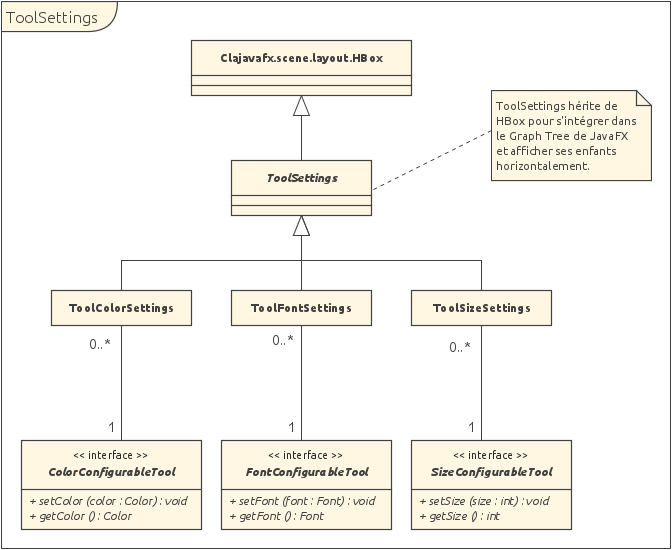
\includegraphics[scale=0.6]{tool_settings.png}
	\label{fig:tool_settings}
\end{figure}

\subsubsection{Pinceau et gomme}
Le pinceau et la gomme ont un comportement et une implémentation quasiment identiques. Dans le programme GEMMS, ce sont les classes Brush et Eraser qui se chargent d'implémenter ces fonctionnalités. Toutes deux héritent d'une classe commune: LineTool. 
\par
Pour ces deux outils, la problématique était la suivante: 
\par 
L'événement MouseDragged est déclenché à intervalles réguliers, tant que l'utilisateur effectue cette action. Pour chaque répétition, il est facile de garder trace de la position de la souris au dernier événement et à l'événement actuel. Connaissant ces deux points, il est possible de dessiner une droite.
\par
Pour ce faire, nous avons utilisé l'algorithme de tracé de segment de Bresenham. Mis au point en 1962, cet algorithme permet de déterminer quels pixels sont à colorer pour relier harmonieusement deux points par une ligne droite.
\par
Il existe de nombreuses implémentations de cet algorithme, et nous avons choisi l'implémentation compacte, que l'on peut trouver sur la page allemande de l'article Wikipédia dédié à ce sujet \cite{Bresenham}.
\par
La classe LineTool se charge donc d'implémenter cet algorithme et pour chaque pixel à colorer, elle appelle une méthode abstraite drawPixel que ses sous classes se chargent de définir. Ainsi, Brush dessiner un disque correspondant à la taille du pinceau, et Eraser efface un carré de pixel, correspondant à la taille de la gomme.
\subsubsection{Pipette}
Le rôle de l'outil pipette et de permettre à l'utilisateur de choisir une couleur en la prélevant sur un élément existant du document. Il s'agirait typiquement de récupérer la couleur d'un calque GEMMSText, GEMMSCanvas ou GEMMSImage.
\par 
Dans le cas d'un texte, la pipette retourne simplement la couleur de celui-ci. Dans le cas d'un objet de type GEMMSCanvas ou d'une GEMMSImage, l'outil lit le pixel exact cliqué par l'utilisateur, ci celui-ci se trouve à l'intérieur des bornes du calque sélectionné.
\subsubsection{Modification de texte}
L'outil de modification de texte permet à l'utilisateur de modifier les propriétés d'un calque texte existant. Lorsque cet outil est activé
\subsubsection{Symétries}
\subsubsection{Déplacement}
\subsubsection{Rotation}
\subsubsection{Redimensionnement}
\subsubsection{Sélection}
\subsubsection{Rognage}





\section{Problèmes connus dans le programme final}
\subsection{Mise-à-jour de l'historique}
Certaines actions ne peuvent pas être détectées par l'historique et donc ne peuvent pas être annulées avec une Ctrl + Z. Notemment, supprimer un calque ou changer son ordre dans la liste des calques. Vu que ces actions sont effectuées directement sur des éléments de la liste observable de JavaFX, situés à plus bas niveau que nos espaces de travail (qui gèrent l'historique), on ne peut pas notifier l'historique après ces actions sans changer notre implémentation.
\subsection{Dessin après redimensionnement et effaçage d'une sélection}

\subsection{Exportation d'une image}
A l'exportation du \texttt{Workspace}, le choix du format de l'image (jpg, png, gif) s'effectue à l'écriture du nom du fichier. Cependant, il n'est pas possible d'afficher des paramètres spécifiques à un format choisi tel que la compression pour le format JPG.

En effet, la classe \texttt{FileChooser} n'est pas spécialisable. Il faudrait donc créer un dialogue \og Exportation d'image \fg{} qui permet gérer tous les formats d'image possible et leurs paramètres. Ceci n'a pas été réalisé par manque de temps et qu'il nous faudrait encore 2 jours pour implémenter cette fonctionnalité. 

\section{Conclusion}

\newpage
\glsaddall
\printglossary[toctitle=Glossaire]

\newpage

%récupérer les citation avec "/footnotemark"
\nocite{*}

%choix du style de la biblio
\bibliographystyle{plain}
%inclusion de la biblio
\bibliography{bibliographie.bib}
%voir wiki pour plus d'information sur la syntaxe des entrées d'une bibliographie

\section{Annexes}
\appendix
    \selectlanguage{french}
    \graphicspath{ {img/} }

    % Page de garde
    \begin{titlepage}
    \begin{center}
        % Upper part of the page. The '~' is needed because only works if a paragraph has started.
        % \includegraphics[width=0.35\textwidth]{./logo}~\\[1cm]
        
        \textsc{\LARGE Haute Ecole d'Ingénierie et de Gestion du Canton de Vaud (HEIG-VD)}\\[1.5cm]
        
        \textsc{\Large }\\[0.5cm]
        
        % Title
        \HRule \\[0.4cm]
        
        {\huge \bfseries Projet de semestre (PRO)\\
            Editeur d'image GEMMS \\[0.4cm] }
        
        \HRule \\[1.5cm]
        
        % Author and supervisor
        \begin{minipage}{0.4\textwidth}
            \begin{flushleft} \large
                \emph{Auteur:}\\
                Edward \textsc{Ransome}\\
                Guillaume \textsc{Milani}\\
                Mathieu \textsc{Monteverde}\\
                Michael \textsc{Spierer}\\
                Sathiya \textsc{Kirushnapillai}
            \end{flushleft}
        \end{minipage}
        \begin{minipage}{0.4\textwidth}
            \begin{flushright} \large
                \emph{Client:} \\
                René \textsc{Rentsch}\\
                \emph{Référent:} \\
                René \textsc{Rentsch}\\
            \end{flushright}
        \end{minipage}
        
        \vfill
        
        % Bottom of the page
        {\large \today}
        
    \end{center}
\end{titlepage}

    \newpage~




    % Espacement entre les lignes d'un tableau
    \renewcommand{\arraystretch}{1.5}

    % Config des pages
    \setlength{\parskip}{1em}
    \setlength{\parindent}{0pt}

    \titlespacing\section{0pt}{12pt plus 4pt minus 2pt}{0pt plus 2pt minus 2pt}
    \titlespacing\subsection{0pt}{12pt plus 4pt minus 2pt}{0pt plus 2pt minus 2pt}
    \titlespacing\subsubsection{0pt}{12pt plus 4pt minus 2pt}{0pt plus 2pt minus 2pt}


    ~
    \thispagestyle{empty}
    % Recommencer la numérotation des pages à "1"
    \setcounter{page}{0}
    \newpage

	\section{Journal de travail - Edward Ransome}

\subsection{Semaine 1 20 février - 24 février}
Création du groupe et recherche d'idées. Discussion et proposition des deux principaux sujets au professeur, un éditeur d'images et un programme de manipulation de graphes.
\subsection{Semaine 2 27 février - 3 mars}
Programme d'édition d'images accepté, début d'élaboration du cahier des charges. Discussion sur le fonctionnement, l'architecture, les fonctionnalités voulues ainsi que des mock-ups d'interface. Travail simultané de tout le groupe.
\subsection{Semaine 3 6 mars - 10 mars}
Fin de rédaction du cahier des charges, avec mock-ups finaux et une liste des fonctionnalités indispensables et optionnelles. Rendu de celui-ci ainsi qu'un planning du travail sous forme de diagramme de Gant.
\subsection{Semaine 4 13 mars - 17 mars}
Retour sur le cahier des charges, pas de problèmes majeurs. Planification rédigée sous forme d'un tableau Excel pour faciliter la compréhension et mieux voir le travail effectué à chaque membre du groupe. Début du travail individuel selon le planning. 
\subsection{Semaine 5 20 mars - 24 mars}
Étude de JavaFX. Tutoriel JavaFX 8 de Code Makery effectué, qui comprends une introduction à Scene Builder, création de fenêtres, effets et autres fonctionnalités de cette librairie. Étude de la documentation Oracle de JavaFX.
\subsection{Semaine 6 27 mars - 31 mars}
Début de création de l'interface avec Guillaume Milani en se basant sur les mock-ups élaborés pour le cahier des charges.
\subsection{Semaine 7 3 avril - 7 avril}
Fin de l'interface Scene Builder avec contrôleurs des boutons dans le code ainsi que des références aux éléments du fichier \og .fxml \fg{} dans le code pour pouvoir les modifier hors de Scene Builder.
\subsection{Semaine 8 10 avril - 14 avril}
Aide à l'implémentation du Workspace dans l'interface graphique principale avec déplacement et zoom.
\subsection{Semaine 9 24 avril - 28 avril}
Continuation de l'implémentation du Workspace dans l'interface.
\subsection{Semaine 10 1 mai - 5 mai}
Début d'élaboration de la zone \og Effet \fg{} de l'interface, recherche sur l'implémentation des effets en JavaFX ainsi que leur application sur divers éléments de la librairie (Image, texte, canvas).
\subsection{Semaine 11 8 mai - 12 mai} 
Création de différents boutons permettant d'augmenter l'opacité, saturation et l'effet sepia. 
\subsection{Semaine 12 15 mai - 19 mai}
Changements dans l'implémentation des effets, un \og Slider \fg{} JavaFX par effet incrémentable, permettant de modifier l'opacité, saturation, contraste et sepia sur un ou plusieurs calques. Implémentation d'une remise à zéro des effets. Début de réfection sur la sérialisation des effets.
\subsection{Semaine 13 22 mai - 26 mai}
Ajout de l'effet de flou, ainsi que un bouton \og Tint \fg{} qui créé une nuance de couleur sur un calque. Implémentation de la sérialisation des effets et correction de l'ordre d'application des effets pour permettre leur application dans un ordre quelconque sans recréer tous les effets.
\subsection{Semaine 14 29 mai - 2 juin}
Finition du rapport et du manuel utilisateur.



 \newpage

    \subsection{Journal de travail - Mathieu Monteverde}

\subsubsection{Semaine 1 20 février - 24 février}
\subsubsection{Semaine 2 27 février - 3 mars}
\subsubsection{Semaine 3 6 mars - 10 mars}
\subsubsection{Semaine 4 13 mars - 17 mars}
\subsubsection{Semaine 5 20 mars - 24 mars}
\subsubsection{Semaine 6 27 mars - 31 mars}
\subsubsection{Semaine 7 3 avril - 7 avril}
\subsubsection{Semaine 8 10 avril - 14 avril}
\subsubsection{Semaine 9 24 avril - 28 avril}
\subsubsection{Semaine 10 1 mai - 5 mai}
\subsubsection{Semaine 11 8 mai - 12 mai}
\subsubsection{Semaine 12 15 mai - 19 mai}
\subsubsection{Semaine 13 22 mai - 26 mai}
\subsubsection{Semaine 14 29 mai - 2 juin}



 \newpage

    \section{Journal de travail - Sathiya Kirushnapillai}

\subsection{Semaine 1 20 février - 24 février}
Constitution des groupes et choix du sujet. De nombreux sujets ont été proposés, la plupart ne faisant pas l'unanimité. Finalement, deux idées ont fait été retenues par le groupe: un programme de manipulation de graphes, et en premier lieu, un programme d'édition d'images.
\subsection{Semaine 2 27 février - 3 mars}
Attribution des sujets de projet. Le projet de programme d'édition d'images a été accepté. Nous avons donc pu commencer la réflexion autour des fonctionnalités et la planification du projet.
\subsection{Semaine 3 6 mars - 10 mars}
Discussion en groupe. Nous faisons le tri des fonctionnalités indispensables et utiles. Une fois celles-ci fixées, nous établissons le cahier des charges et la planification Gant qui va avec.
\subsection{Semaine 4 13 mars - 17 mars}
Le professeur nous fourni un retour sur notre cahier des charges et notre planification. Pour plus de clarté, nous remplissons une nouvelle planification dans un format Excel. Nous nous mettons d'accord sur le fait de prendre deux semaines pour étudier la technologie JavaFX que nous utiliserons pour le projet et qu'aucun de nous ne connaît.
\subsection{Semaine 5 20 mars - 24 mars}
Étude de JavaFX.
\subsection{Semaine 6 27 mars - 31 mars}
Étude de JavaFX. Début de la mise en place de la structure de la classe Workspace avec la spécification des méthodes. Nous réalisons également que des difficultés sont à attendre pour la gestion des calques, de la sérialisation et des éléments issus de JavaFX en général.
\subsection{Semaine 7 3 avril - 7 avril}
Implémentation du Workspace avec insertion et suppression de calques.
\subsection{Semaine 8 10 avril - 14 avril}
Implémentation de la gestion du Workspace pour le déplacement et le zoom de l'utilisateur dans l'interface. Premières recherches pour la gestion de calques au moyen d'une ListView de JavaFX.
\subsection{Semaine 9 24 avril - 28 avril}
Ajout des prototypes recherchés en semaine 9 au reste du projet. Le Workspace permet maintenant d'ajouter des calques, de les supprimer, et de se déplacer dans l'interface. 
\subsection{Semaine 10 1 mai - 5 mai}
Des changements ont eu lieu pour le Workspace. De mon côté, il faut encore améliorer la gestion des calques.
On se rend compte que l'élément ListView de JavaFX, qui pourrait pourtant de fonctionner parfaitement pour l'affichage des calques, ne permet de pas de changer l'ordre d'affichage.
\subsection{Semaine 11 8 mai - 12 mai} 
Il va falloir trouver une solution pour la gestion des calques. Le module étant cependant fonctionnel, on se charge des autres fonctionnalités. Début de la réalisation du pinceau et de la gomme.
\subsection{Semaine 12 15 mai - 19 mai}
Remplacement de la ListView de gestion des calques JavaFX par un composant fait main pour pouvoir répondre aux besoins de l'application. Les outils pinceaux, gommes et pipette sont fonctionnels. Beaucoup d'élément ont pu être ajoutés cette semaine. La gestion de la couleur, le paramétrage des outils (taille du pinceau et de la gomme, édition de textes et autres).
\subsection{Semaine 13 22 mai - 26 mai}
Il y a eu beaucoup de problèmes avec les transformations de calques (rotation, taille, symétrie, etc.) Mais après beaucoup d'efforts, les problèmes ont pu être résolu. Maintenant, il s'agit de peaufiner l'interface (espacement, ergonomie, retour visuels pour l'utilisateur, etc.),
\subsection{Semaine 14 29 mai - 2 juin}
Finition du rapport et du manuel utilisateur.



 \newpage

    \section{Journal de travail - Michael Spierer}

\subsection{Semaine 1: 20 février - 24 février}
Nous avons constitué notre groupe et fait un brainstorming afin de trouver des idées. Nous retenons les deux meilleures afin de les proposer pour le projet.
\subsection{Semaine 2: 27 février - 3 mars}
Notre idée de faire un éditeur d'images a été accepté et nous avons pu commencer à écrire le cahier des charges et à trouver quelles fonctionnalités nous voulons avoir.
\subsection{Semaine 3: 6 mars - 10 mars}
Cahier des charges final et planification Gantt. Cette dernière prend pas mal de temps car un editeur d'image, d'après les conseils de Mr Rentsch aux vues des dernières années, amène beaucoup d'interdépendance au sein d'un groupe.
\subsection{Semaine 4: 13 mars - 17 mars}
Notre Gantt étant trop complexe niveau compréhension, on nous demande de le refaire sur Excel afin de le rendre plus claire. 
\subsection{Semaine 5: 20 mars - 24 mars}
Étude de JavaFX, tests de certaines fonctionnalitées de JavaFX, tutoriels de base de JavaFX.
\subsection{Semaine 6: 27 mars - 31 mars}
Étude de JavaFX, tests de certaines fonctionnalitées afin de jeter un coup d'oeil aux fonctionnalitées que je vais devoir implémenter par la suite.
\subsection{Semaine 7: 3 avril - 7 avril}
Début d'implémentation du Workspace.
\subsection{Semaine 8: 10 avril - 14 avril}
Recherche de la gestion de calques avec Mathieu, on rencontre déjà des problèmes qui vont nous faire nous poser pas mal de questions, par exemple, un Node n'est pas sérialisable, donc on essaie de trouver des solutions à ce problème.
\subsection{Semaine 9: 24 avril - 28 avril}
Gestions de calques avec Mathieu. On a fait en sorte de rendre les calques ( n\oe uds) sérialisables (on a ajouté des méthodes pour sérialiser et desérialiser avec l'aide de Sathiya car il avait déjà bossé sur la question de la sérialisation). On peut ajouter nos calques personnels (GEMMSImage par exemple) au workspace.
\subsection{Semaine 10: 1 mai - 5 mai}
Implémentation des calques de texte (GEMMSText) et leurs outils de modifications,(taille, etc.).
\subsection{Semaine 11: 8 mai - 12 mai} 
Redimensionnement des calques, pivotement, deplacement d'un ou plusieurs calques. Il y a plusieurs manières d'aboutir aux effets escomptés, plusieurs choses rentrent en compte : vu que quasiment rien n'est sérialisable, il faut trouver comment sérialiser les transformations, en plus de sérialiser les calques qui sont de base non-sérialisable.
\subsection{Semaine 12: 15 mai - 19 mai}
Toujours sur les outils de transformations de n\oe uds. Il y a de nouveau soucis : le mappage de coordonnées des tools (pas juste les transformations que j'implémente mais aussi brush etc) ne se fait pas bien. Pour finir, on parvient à regler le soucis. De plus, les symetries m'ont donné du fil à retordre mais marchent parfaitement en fin de compte. Ces symetries ne sont pas extremement dure niveau code mais on amené pas mal de problème interne, par exemple niveau sérialisation ou transformation.
\subsection{Semaine 13: 22 mai - 26 mai}
Implémentation de l'alignement automatique avec effet aimant d'un calque lors de son déplacement.
Essaie de faire un bonus qui n'est pas dans le cahier des charges pour la réalisation d'un bucket (afin de remplir une zone d'une couleur en un clique). Le prototype marche bien sauf à partir du moment où il y a une transformation sur le calque. Je reévalue la situation, pas de temps à perdre sur cette fonctionnalité non demandée, je passe à la suite. Implémentation de l'alignement automatique d'un calque lors du drag.
\subsection{Semaine 14: 29 mai - 2 juin}
Rapport et journal de bord.





 \newpage

    \section{Journal de travail - Guillaume Milani}

\subsection{Semaine 1: 20 février - 24 février}
Constitution des groupes et choix du sujet. Le choix du sujet n'est pas facile, plusieurs idées sont proposées et un vote doit avoir lieu. Au final nous proposerons un projet de résolution de graphe et un éditeur d'images.
\subsection{Semaine 2: 27 février - 3 mars}
Les sujets sont attribués, le projet d'éditeur d'image est préféré car un autre groupe est aussi intéressé par l'éditeur de graphe. Nous commençons la liste des fonctionnalités à proposer et l'écriture du cahier des charges.
\subsection{Semaine 3: 6 mars - 10 mars}
Nous fixons la liste des fonctionnalités que nous souhaitons voir apparaître dans notre programme. Nous rédigeons le cahier des charges ainsi que la planification Gantt (très importante car notre projet sera basé presque entièrement sur une seule et unique vue, interface).
\subsection{Semaine 4: 13 mars - 17 mars}
À la demande de M. Rentsch, nous remplissons une planification au format Excel, plus claire que le Gantt précédemment. Nous commençons l'étude de JavaFX chacun de notre côté, il s'agit pour nous d'une première expérience avec ce Framework.
\subsection{Semaine 5: 20 mars - 24 mars}
Étude de JavaFX et création des issues sur Github que nous utiliserons par la suite. Je reproduis la planification sous forme de Milestones et attribue chaque issue aux personnes concernées.
\subsection{Semaine 6: 27 mars - 31 mars}
Début de la création de l'interface de l'application à l'aide de l'outil Scene Builder en essayant de reproduire à l'identique la maquette présentée dans le cahier des charges.
\subsection{Semaine 7: 3 avril - 7 avril}
Edward et moi-même mettons en place le contrôleur Java qui interagira avec la vue au formal FXML.
\subsection{Semaine 8: 10 avril - 14 avril}
Commentaire du contrôleur et mise en place d'un fonction pour générer dynamiquement les boutons des outils afin de faciliter le travail des autres membres de l'équipe.
\subsection{Semaine 9: 24 avril - 28 avril}
Documentation sur les Popups, implémentation d'un popup qui permettra de modifier la taille et la couleur d'un outil. Ce popup sera finalement abandonné par la suite pour simplifier l'interface.
\subsection{Semaine 10: 1 mai - 5 mai}
Réflexion sur la manière d'effectuer le copier / coller. Je dois d'abord parcourir et comprendre le code de Sathiya qui a mis en place la sélection d'une zone de l'espace de travail ainsi que la sérialisation des calques.

Je rencontre des problèmes pour enregistrer une capture de l'espace de travail, je ne comprend pas bien comment les couleurs sont gérées lors de la création d'une image.
\subsection{Semaine 11: 8 mai - 12 mai}
Une première version du copier / coller est implémentée et fonctionne avec quelques problèmes (le calque collé ne se place pas au bon endroit). J'ai résolu les problèmes de couleur et de copie d'image en copiant les pixels un à un et en ne copiant pas les pixels transparents, pour éviter une conversion en blanc.
\subsection{Semaine 12: 15 mai - 19 mai}
Les problèmes de placement du calque collé sont résolus. Il faut être attentif au système de coordonnées que l'on utilise lorsqu'on exécute un snapshot et ne pas oublier de convertir les coordonnées au besoin.

La fonction copier / coller est fonctionnelle, commentée et nettoyée au mieux.
\subsection{Semaine 13: 22 mai - 26 mai}
Implémentation de la fonction d'historique. Malgré une réflexion sur le sujet depuis le début de la phase d'implémentation en mars, je n'aurai pas le temps d'implémenter la version «efficace» qui consisterait à enregistrer chaque action et une fonction permettant de l'inverser. J'opte donc pour la solution plus facile à mettre en place qui consiste à enregistrer l'état de l'espace de travail après chaque action de l'utilisateur.

En milieu de semaine l'historique fonctionne et je commence à implémenter la partie «visuelle» qui permettra d'afficher les miniatures dans l'interface de l'application.
\subsection{Semaine 14: 29 mai - 2 juin}
Fin de la partie visuelle de l'historique et rédaction du rapport.
 \newpage


\end{document}
